\begin{frame}\begin{center}
		\LARGE\textbf{Mathematical models}
\end{center}\end{frame}
%-------------------------------------------------------------------------------
%-------------------------------------------------------------------------------
\begin{frame}\textbf{Lecture}\vspace{0.3cm}

All models are designed to shed light on the process of schooling decisions.\\\vspace{0.3cm}

\begin{itemize}\setlength\itemsep{1em}
\item Compensating differences
\item Accounting-identity
\item Option value
\end{itemize}

\end{frame}
%-------------------------------------------------------------------------------
%-------------------------------------------------------------------------------
\begin{frame}
Economic models facilitate experiential learning.\vspace{0.3cm}
\begin{itemize}\setlength\itemsep{1em}
\item What question are they designed to address?
\item What are the underlying economic mechanisms?
\item How robust are the conclusions?
\item What is missing?
\item $\hdots$
\end{itemize}

\end{frame}
%-------------------------------------------------------------------------------
%-------------------------------------------------------------------------------
\begin{frame}
	\begin{figure}[htp]\centering
		\caption{Modeling process}\scalebox{0.45}
		{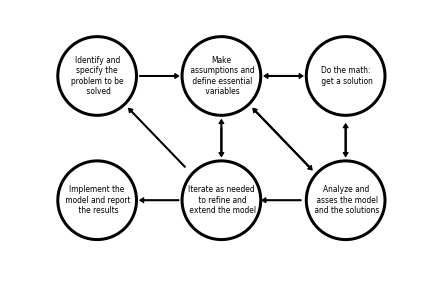
\includegraphics{fig-modeling-process}}
	\end{figure}
\end{frame}
%-------------------------------------------------------------------------------
%-------------------------------------------------------------------------------
